\documentclass[11pt, oneside]{article}   	% use "amsart" instead of "article" for AMSLaTeX format
\usepackage{geometry}                		% See geometry.pdf to learn the layout options. There are lots.
\geometry{letterpaper}                   		% ... or a4paper or a5paper or ... 
%\geometry{landscape}                		% Activate for rotated page geometry
%\usepackage[parfill]{parskip}    		% Activate to begin paragraphs with an empty line rather than an indent
\usepackage{graphicx}				% Use pdf, png, jpg, or eps§ with pdflatex; use eps in DVI mode
								% TeX will automatically convert eps --> pdf in pdflatex		
\usepackage{amssymb}

\usepackage{listings} 
\usepackage{color}
\definecolor{dkgreen}{rgb}{0,0.6,0}

\lstset{
   breaklines=true,                                     % line wrapping on
   language=SQL,
   %frame=ltrb,
   framesep=5pt,
   basicstyle=\normalsize,
   %keywordstyle=\ttfamily\color{OliveGreen},
   %identifierstyle=\ttfamily\color{CadetBlue}\bfseries,
   commentstyle=\color{dkgreen},
   stringstyle=\ttfamily,
   showstringspaces=ture
}

% Add your keywords here, and have this in a separate file
% and include it in your preamble
\lstset{emph={ 
    DATETIME, REFERENCES
    },emphstyle={\textbf}
}


\title{CS 660: Project Assignment \#1}
\author{Bowen Zhang (U881677028) \\Yiwen Gu (U58170649)}
\date{}							% Activate to display a given date or no date

\begin{document}
\maketitle
\section{The ER-Diagram}				
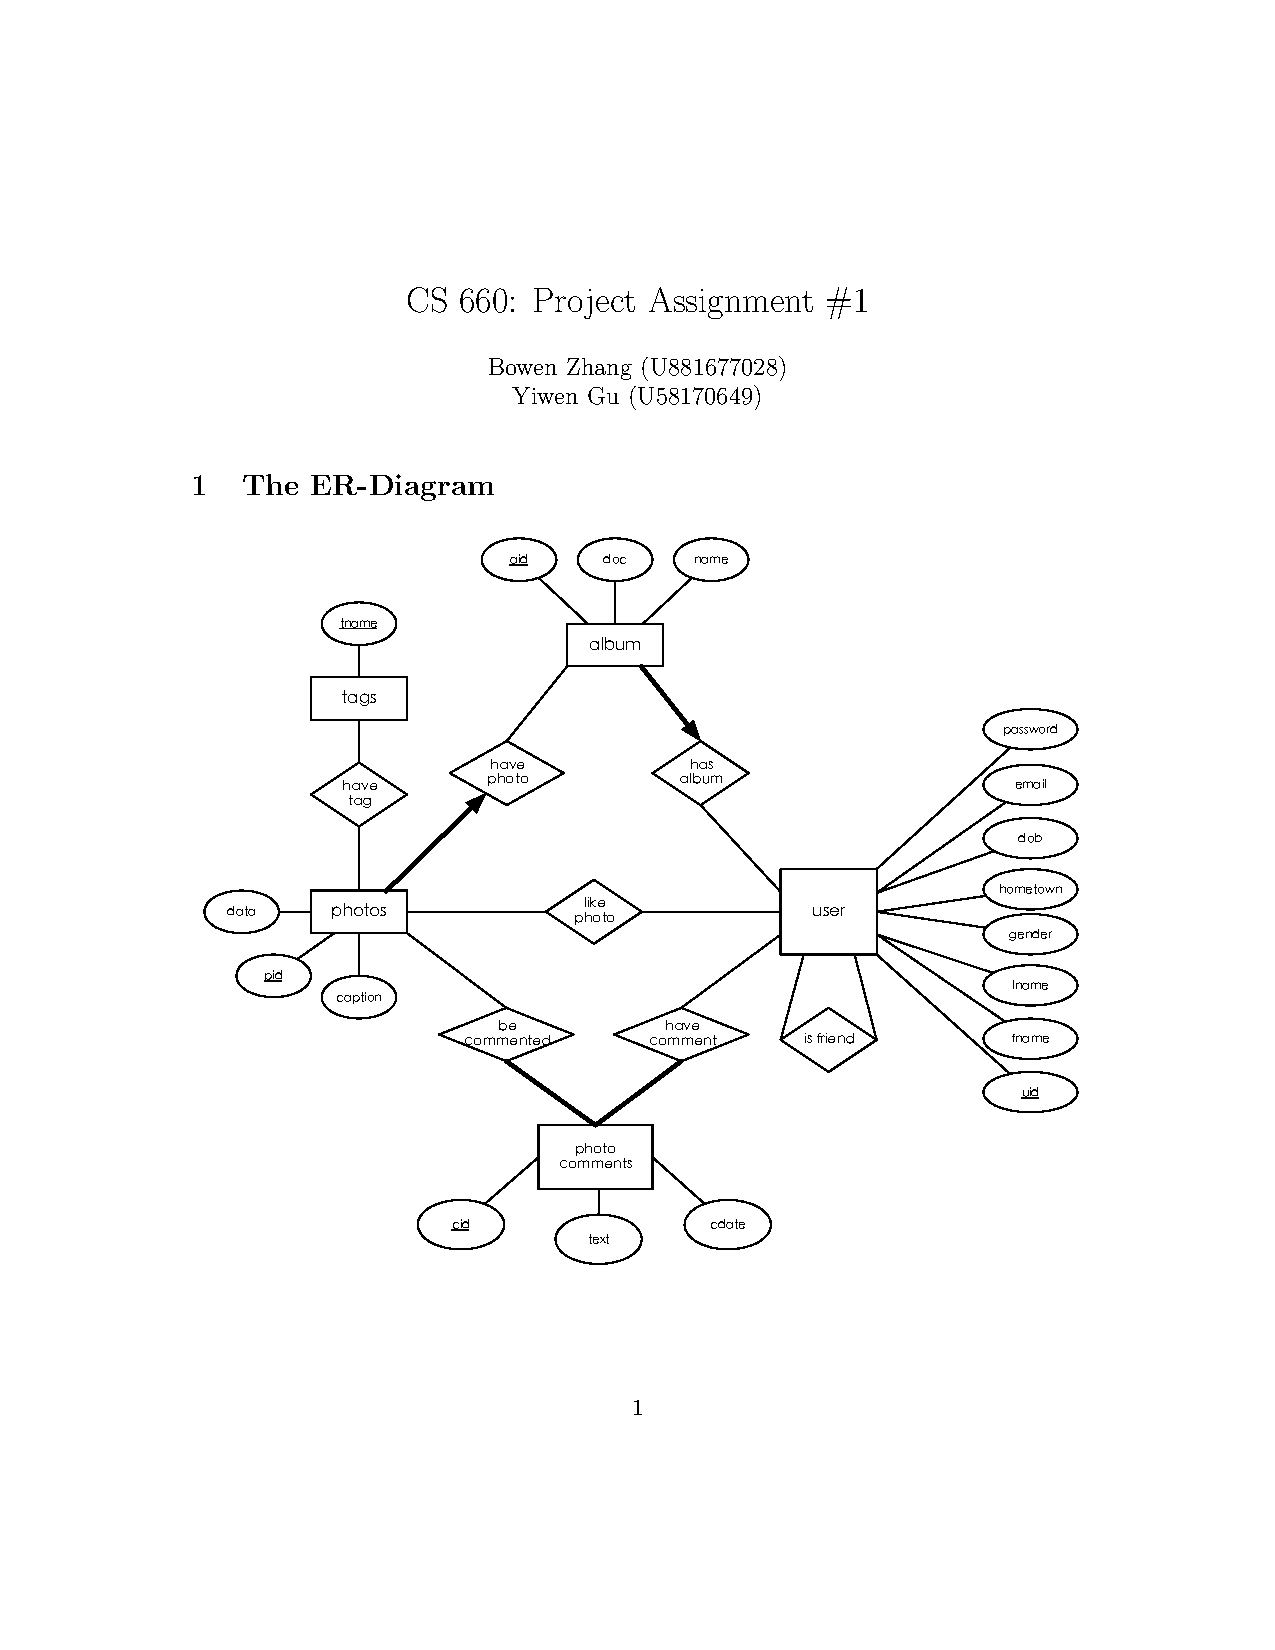
\includegraphics[width=6in]{pa1.png} 

\section{The Schema}
\begin{lstlisting}[frame=none]		 	% Start the code-block SQL

CREATE TABLE User(
   uid  INTEGER,
   fname  VARCHAR(20),
   lname  VARCHAR(20),
   email  VARCHAR(50),
   dob  DATE,
   hometown  VARCHAR(20),
   gender  CHAR(1),
   password  VARCHAR(20),
   PRIMARY KEY  (uid),
   UNIQUE (email)
   );

CREATE TABLE Album(
   aid  INTEGER,
   name  VARCHAR(20),
   cdate  DATETIME,
   uid INTEGER NOT NULL,
   PRIMARY KEY  (aid),
   FOREIGN KEY (uid) REFERENCES User(uid)
  	ON DELETE NO ACTION
   );
/* Assumption: each album has to belong to one user */

CREATE TABLE Photos(
   pid  INTEGER,
   caption  VARCHAR(200),
   data LONGBLOB,
   PRIMARY KEY  (pid),
   FOREIGN KEY (aid) REFERENCES Album(aid)
  	ON DELETE NO ACTION
   );
/* Assumption: each photo has to belong to one album, 
   a photo copied from one album to another will have its 
   own (different) pid. */

CREATE TABLE Tags(
   tname  VARCHAR(50),
   pid INTEGER,
   PRIMARY KEY  (tname),
   FOREIGN KEY (pid) REFERENCES Photos(pid)
   );

CREATE TABLE isFriend(
   uid  INTEGER,
   fuid  INTEGER,
   PRIMARY KEY  (uid, fuid),
   FOREIGN KEY  (uid) REFERENCES User(uid),
   FOREIGN KEY  (fuid) REFERENCES User(uid),
   CHECK (uid <> fuid)
   );
/* Assumption: a user cannot be friend to him/herself;  
   (A,B) and (B,A) are different in this table */

CREATE TABLE Comments(
   cid  INTEGER,
   cdate  DATETIME,
   text  VARCHAR(255),
   pid  INTEGER NOT NULL,
   uid  INTEGER NOT NULL, 
   PRIMARY KEY  (cid),
   FOREIGN KEY  (pid) REFERENCES Photos(pid),
   FOREIGN KEY  (uid) REFERENCES User(uid)
   );

CREATE TABLE likePhoto(
   uid  INTEGER,
   pid  INTEGER,
   PRIMARY KEY  (uid, pid),
   FOREIGN KEY  (uid) REFERENCES User(uid),
   FOREIGN KEY  (pid) REFERENCES Photos(pid)
   );

\end{lstlisting}


\section{The Constrains}
The entity set \textbf{Album} has a key constraint in the relationship set \textbf{hasAlbum}.\\
The entity set \textbf{Photos} has a key constraint in the relationship set \textbf{havePhoto}.














\end{document}  